\documentclass[12pt,a4paper,UTF8]{ctexart}
\usepackage{graphicx}
\usepackage{amsmath}
\usepackage{amssymb}
\usepackage{subfig}
\usepackage{cite}
\usepackage[ntheorem]{empheq}
\usepackage{enumitem}
\usepackage{fullpage}
\usepackage{cleveref}
\usepackage{cellspace}
\usepackage{listings}
\usepackage{color}
\definecolor{gray}{rgb}{0.5,0.5,0.5}
\definecolor{dkgreen}{rgb}{.068,.578,.068}
\definecolor{dkpurple}{rgb}{.320,.064,.680}

% set Matlab styles
\lstset{
   language=Matlab,
   keywords={break,case,catch,continue,else,elseif,end,for,function,
      global,if,otherwise,persistent,return,switch,try,while},
   basicstyle=\ttfamily,
   keywordstyle=\color{blue}\bfseries,
   commentstyle=\color{dkgreen},
   stringstyle=\color{dkpurple},
   backgroundcolor=\color{white},
   tabsize=4,
   showspaces=false,
   showstringspaces=false
}

\begin{document}
\CJKfamily{zhkai}	


\begin{center}
\textbf{作业三}\\
\textbf{姓名: ~~马宇骁~~~~~~~~ 学号 :~~~PB19151769~~~~~~~~ 日期:~~\today}\\
\end{center}

\begin{center}
\fbox{
\begin{minipage}{40em}
\vspace{5cm}
\hspace{20cm}
\end{minipage}}
\end{center}
\vspace{1cm}

\begin{enumerate}
\item[第一题] 

(a)

\textsc{Matlab}程序显示如下:
\begin{lstlisting}[frame=single]
clear,clc
for k = 0:15
    h = 10^(-k);
    fx = fdiff(1.2,h);
    labels(k+1,1) = h;
    labels(k+1,2) = abs(fx-cos(1.2));
end
hchange(labels);

function fx = fdiff(x0,h)
syms x;
f(x) = sin(x);
fx = (f(x0+h)-f(x0))/h;
end
function hchange(labels)
loglog(labels(:,1),labels(:,2));
% 记录横轴纵轴的数据画图
xlabel('h');
ylabel('精度');
grid on;
legend
end
\end{lstlisting}
\begin{center}
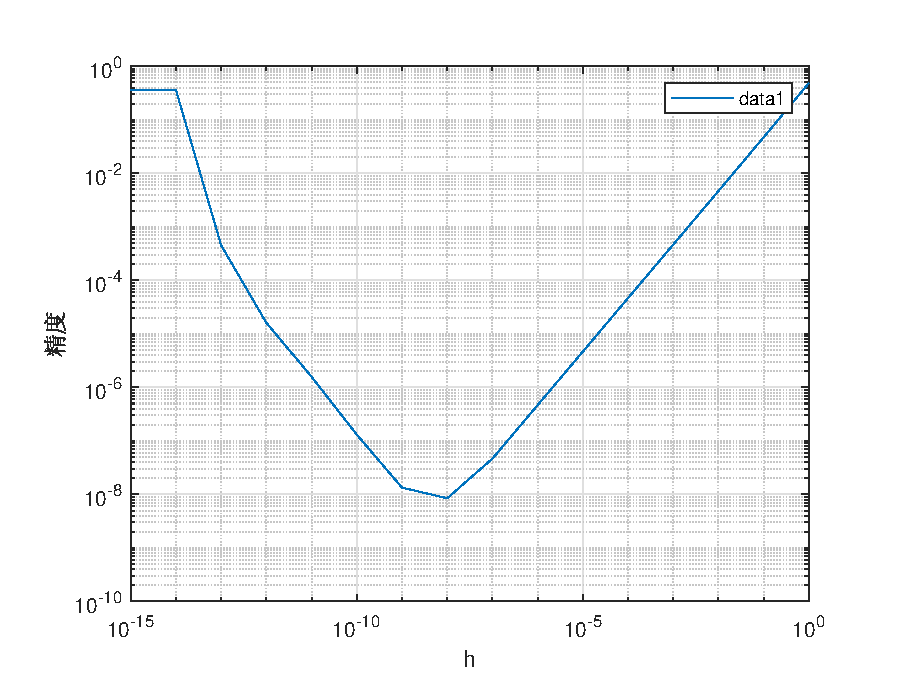
\includegraphics[scale=1]{1a.eps}
\end{center}

(b)

\qquad $f(x_0) = f(x_0)$ \hfill (1)

\qquad $f(x_0 + h) = f(x_0) + hf'(x_0) + \frac{h^2}{2!} f''(x_0) + O(h^3)$ \hfill (2)

\quad 由((2) - (1)) / h 得:

\quad $\Rightarrow f'(x_0) = \frac{f(x_0 + h) - f(x_0)}{h} - \frac{h}{2!} f''(x_0) + O(h^2)$

\quad 记$N_1(h) = \frac{f(x_0 + h) - f(x_0)}{h}$,

\qquad $f'(x_0) = N_1(h) - \frac{h}{2!} f''(x_0) + O(h^2)$ \hfill (3)

\qquad $f'(x_0) = N_1(\frac{h}{2}) - \frac{1}{2}(\frac{h}{2!}) f''(x_0) + O(h^2)$ \hfill (4)

\quad 2*(4) - (3)得:

\qquad $f'(x_0) = 2N_1(\frac{h}{2}) - N_1(h) + O(h^2) \approx N_2(h)$

\qquad $N_2(h) = 2N_1(\frac{h}{2}) - N_1(h)$

\quad 继续外推:

for j = 2 : n

\qquad $N_j(h) = 2N_{j-1}(\frac{h}{2}) - N_{j-1}(h)$ 

\qquad $f'(x_0) = N_j(\frac{h}{2})$

end

(c)

\textsc{Matlab}程序显示如下:
\begin{lstlisting}[frame=single]
for n = 0:14
    disp(n);
    h0 = 2^(-n);
    nearest = RFD(h0); 
    N(n+1,1) = nearest;
    hold on
end
N
function nearest = RFD(h0)
eps = 1e-15;
%设置误差界
syms x;
syms h;
x0 = 1.2;
f(x) = sin(x);
N(h) = (f(x0+h)-f(x0))/h;
k0 = 1;
d = double(abs(N(h0)-N(h0/2)));
fx = double(N(h0));
labels(1,1) = 1;
labels(1,2) = abs(fx - cos(1.2));
for k0 = 2: 100
    if d<=eps || abs(fx - cos(1.2))<=eps
        break;
    else
        N(h) = 2*N(h/2)-N(h);
        d = double(abs(N(h0)-N(h0/2)));
        fx = double(N(h0));
        labels(k0,1) = k0;
        labels(k0,2) = abs(fx - cos(1.2));
        labels(k0,3) = fx;
    end
end
[Y,I] = min(labels,[],1);
nearest = labels(I(1,2),3);
name1 = ['h0 =',num2str(h0)];
semilogy(labels(:,1),labels(:,2),'DisplayName',name1);
% 记录横轴纵轴的数据画图
name2 = [' \leftarrow ',name1]; %w 的数字指向线
text(5,labels(5,2),name2);
xlabel('外推次数');
ylabel('精度');
legend
end
\end{lstlisting}
\begin{flushleft}
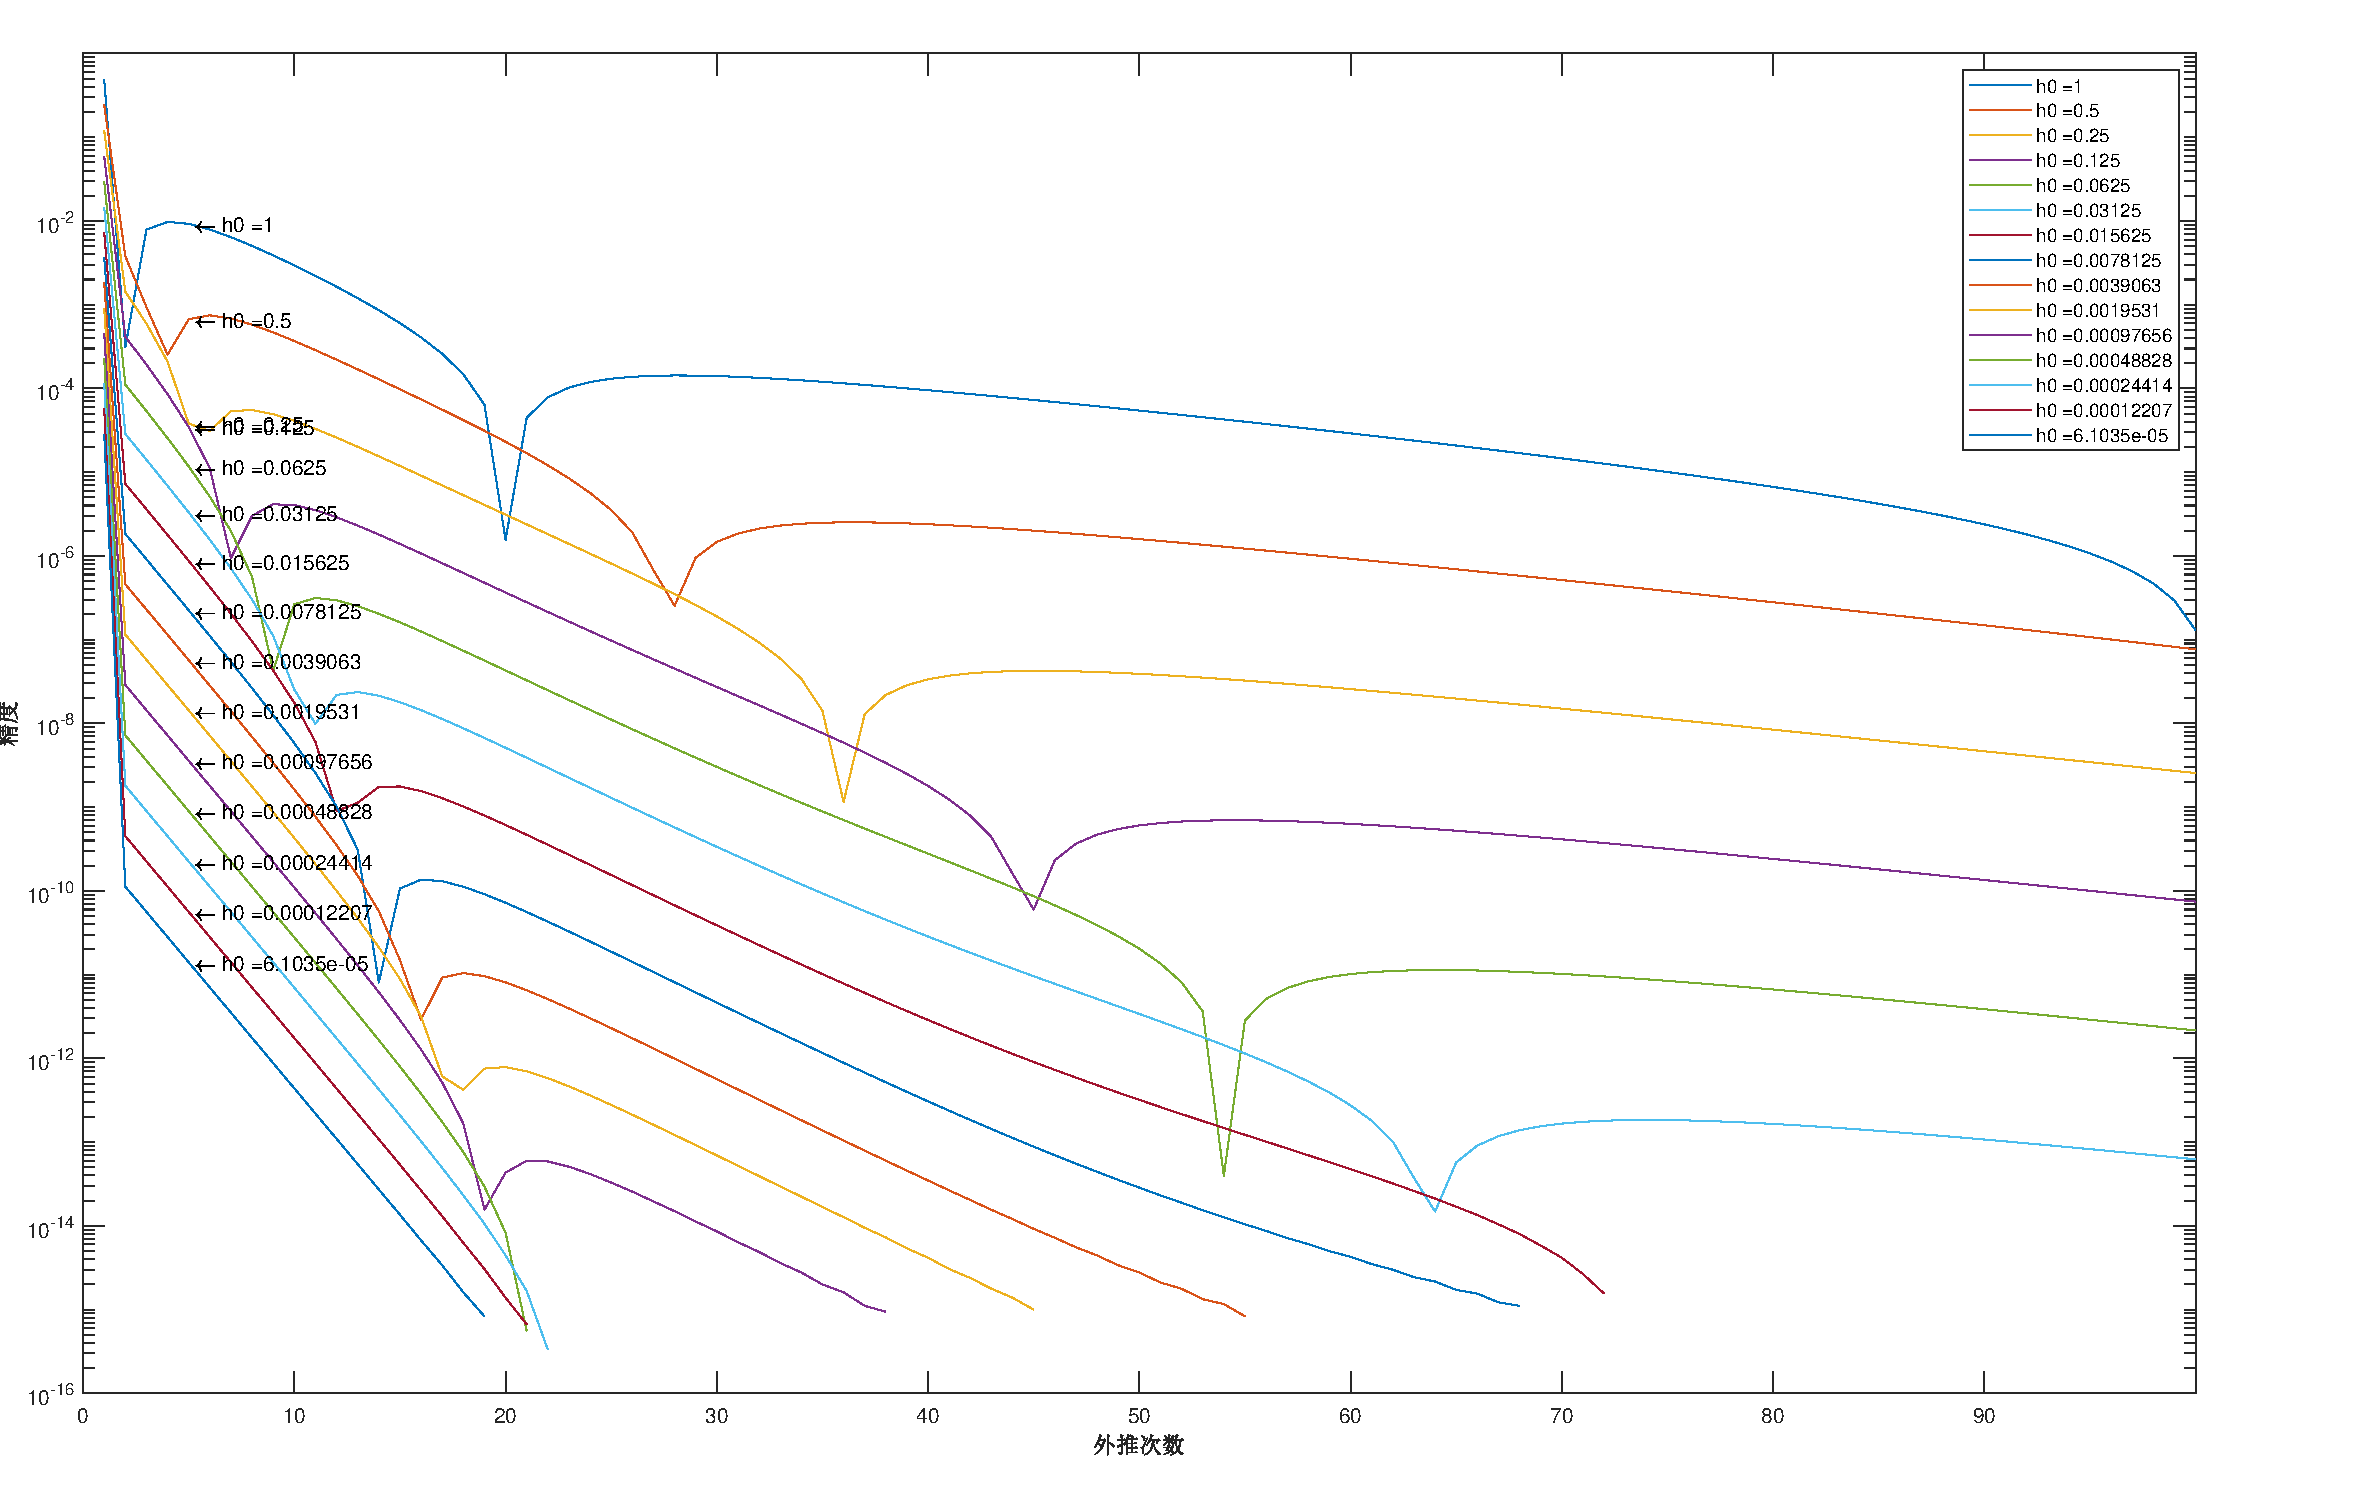
\includegraphics[scale=0.4]{1c.eps}
\end{flushleft}
N =
    0.362357883861802
    0.362357831111555
    0.362357755629859
    0.362357754416836
    0.362357754476634
    0.362357754476688
    0.362357754476672
    0.362357754476673\\
    0.362357754476674
    0.362357754476675
    0.362357754476673
    0.362357754476674\\
    0.362357754476674
    0.362357754476673
    0.362357754476673

\item[第二题] 

(a)

\qquad $h = \frac{b - a}{h} = \frac{2\pi}{m}$

\qquad $I = \sum_{k = 0}^{n} A_kf(x_k)$

\qquad $T_n = \frac{h}{2} \sum_{k = 1}^{n} (f(x_k)+f(x_{k-1})) = \frac{h}{2}(f(a) + f(b) + 2\sum_{k = 1}^{n-1}f(x_k))$

\qquad $E_{T_n} = I - I_n = -\frac{h^3}{12}\sum_{k = 0}^{n-1}f''(\eta_k) = -\frac{b-a}{12}h^2f''(\eta)$

%\qquad $E_{S_n} = I - S_n = -\frac{h^5}{2880}\sum_{k = 0}^{n-1}f^{(4)}(\eta_k)$

%\qquad \qquad $ = -\frac{b-a}{2880}h^4f^{(4)}(\eta)$

由此,带入已知条件:

(1)

\quad $\Rightarrow |E| = |\frac{2\pi}{12}\frac{(2\pi)^2}{m^2}(cos r\eta)^{(2)}| = |\frac{3\pi^3}{4m^2} r^2 cosr\eta| \leq \frac{3\pi^3 r^2}{4m^2}$

\quad $r = km$时,$|E| \leq \frac{3\pi^3 k^2}{4}$


(2)

\quad $\Rightarrow |E| = |\frac{2\pi}{12}\frac{(2\pi)^2}{m^2}(sin r\eta)^{(2)}| = |\frac{3\pi^3}{4m^2} r^2 sinr\eta| \leq \frac{3\pi^3 r^2}{4m^2}$

\quad $r = km$时,$|E| \leq \frac{3\pi^3 k^2}{4}$

故,误差都有界,因此能提高精度。

\textsc{Matlab}(b)程序显示如下:
\begin{lstlisting}[frame=single]
err = 1;
m = 1;
while err>= 1e-15
    disp(m);
    err = intg(m);
    labels(m,1) = m;
    labels(m,2) = err;
    m = m+1;
end
errors(labels);

function err = intg(m)
syms x;
f(x) = exp(cos(x));
h = 2*pi/m;
T = 0;
for k = 1:m
    T = T + h/2*(f(-pi+k*h)+f(-pi+(k-1)*h));
end
ext = 7.954926521012845274513219665329394328161342771816638
      573400595955383360608164694666995137357228568774;
      %用Wolfram alpha的在线计算器算得
err = abs(ext - T);
end
function errors(labels)
semilogy(labels(:,1),labels(:,2),'DisplayName','精度图');
% 记录横轴纵轴的数据画图
xlabel('m');
ylabel('精度');
grid on;
legend
\end{lstlisting}
\begin{center}
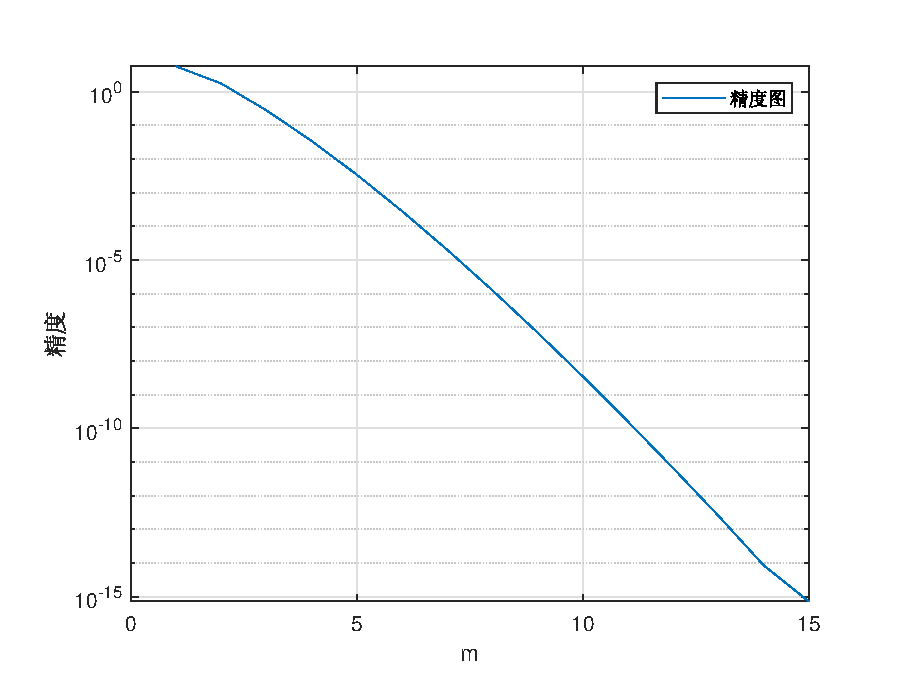
\includegraphics[scale=1]{2b.eps}
\end{center}

\item[第三题]

(a)

令$y'(t) = f(t,y(t))$,

$\Rightarrow y(t_n) = y(t_{n-p}) + \int_{t_{n-p}}^{t_n} f(t,y(t))dt$

用Lagrange插值多项式近似$f(t,y(t))$,

$y(t_n) = y(t_{n-p}) + \int_{t_{n-p}}^{t_n} L_{n-q}^n(t)dt$

其中,$L_{n-q}^n(t)dt = \sum_{k = n-q}^{n} f_kl_k(t)$

$f_k = f(t_k,y_k)$

$\Rightarrow y_n = y_{n-p} + \sum_{k = n-q}^{n} f_k \int_{t_{n-p}}^{t_n} l_k(t)dt$

当 p = 2, n = n+1时,

$y_{n+1} = y_{n-1} + f_{n-1}\int_{t_{n-1}}^{t_n+1} l_{n-1}(t)dt + f_{n}\int_{t_{n-1}}^{t_n+1} l_{n}(t)dt + f_{n+1}\int_{t_{n-1}}^{t_n+1} l_{n+1}(t)dt$

其中,记步长为$h$,

$\int_{t_{n-1}}^{t_n+1} l_{n-1}(t)dt = \int_{t_{n-1}}^{t_n+1} \frac{(t-t_{n})(t-t_{n+1})}{(t_{n-1}-t_{n})(t_{n-1}-t_{n+1})}dt = \frac{1}{3}h$

$\int_{t_{n-1}}^{t_n+1} l_{n}(t)dt = \int_{t_{n-1}}^{t_n+1} \frac{(t-t_{n-1})(t-t_{n+1})}{(t_{n}-t_{n-1})(t_{n}-t_{n+1})}dt = \frac{4}{3}h$


$\int_{t_{n-1}}^{t_n+1} l_{n+1}(t)dt = \int_{t_{n-1}}^{t_n+1} \frac{(t-t_{n-1})(t-t_{n})}{(t_{n+1}-t_{n-1})(t_{n+1}-t_{n})}dt = \frac{1}{3}h$

$\Rightarrow y_{n+1} = y_{n-1} + \frac{h}{3}f_{n+1} + \frac{4h}{3}f_n + \frac{h}{3}f_{n-1}$
\\

(b)

若$y_{n-1} = y(x_{n-1}), y_n = y(x_n), y_{n+1} = y(x_{n+1})$,则有:

$y_{n+1} = y(x_{n-1}) + \frac{h}{3}f_{n+1} + \frac{4h}{3}f_n + \frac{h}{3}f_{n-1}$

依微分方程有:

$y_{n+1} = y(x_{n-1}) + \frac{h}{3} (y'(x_{n+1}) + 4y'(x_n) + y'(x_{n-1}))$

$T_{n+1} = y(x_{n+1}) - y_{n+1} = y(x_{n+1}) - y(x_{n-1}) - \frac{h}{3} (y'(x_{n+1}) + 4y'(x_n) + y'(x_{n-1}))$

$y(x_{n+1}) = y(x_{n}) + hy'(x_{n}) + \frac{h^2}{2!}y''(x_n) + \frac{h^3}{3!}y'''(x_n) + O(h^4)$

$y(x_{n-1}) = y(x_{n}) - hy'(x_{n}) + \frac{h^2}{2!}y''(x_n) - \frac{h^3}{3!}y'''(x_n) + O(h^4)$

$y'(x_{n+1}) = y'(x_{n}) + hy''(x_{n}) + \frac{h^2}{2!}y'''(x_n) + O(h^3)$

$y'(x_{n-1}) = y'(x_{n}) - hy''(x_{n}) + \frac{h^2}{2!}y'''(x_n) - O(h^3)$

带入得,

$T_{n+1} = O(h^4)$

$\Rightarrow$ 三阶格式


\textsc{Matlab}(c)程序显示如下:
\begin{lstlisting}[frame=single]
clear,clc
syms x;
syms y;
f(x,y) = x*exp(-4*x) - 4*y;
h = 2/1000;
%步长2/1000
y0 = 0;
k1 = f(0,0);
y1 = y0 + h*f(h/2,h/2 * k1);
k11 = f(h,h);
y2 = y1 + h*f(h+h/2,y1+h/2 * k11);
labels(1,1) = 0;
labels(1,2) = y0;
labels(2,1) = h;
labels(2,2) = y1;
labels(3,1) = h+h;
labels(3,2) = y2;
for k = 4:1001
    yk = labels(k-2,2) + h/3 *(7*f((k-2)*h,labels(k-1,2))- 
         2*f((k-3)*h,labels(k-2,2))+ f((k-4)*h,labels(k-3,
         2)));
    yk = labels(k-2,2) + h/3 *(f((k-1)*h,yk) + 4*f((k-2)*h,
         labels(k-1,2)) + f((k-3)*h,labels(k-2,2)));
    labels(k,1) = (k-1)*h;
    labels(k,2) = yk;
    disp(k);
end
fx(labels);
function fx(labels)
semilogy(labels(:,1),labels(:,2),'DisplayName','解函数');
% 记录横轴纵轴的数据画图
xlabel('x');
ylabel('y');
grid on;
legend
end
\end{lstlisting}
\begin{center}
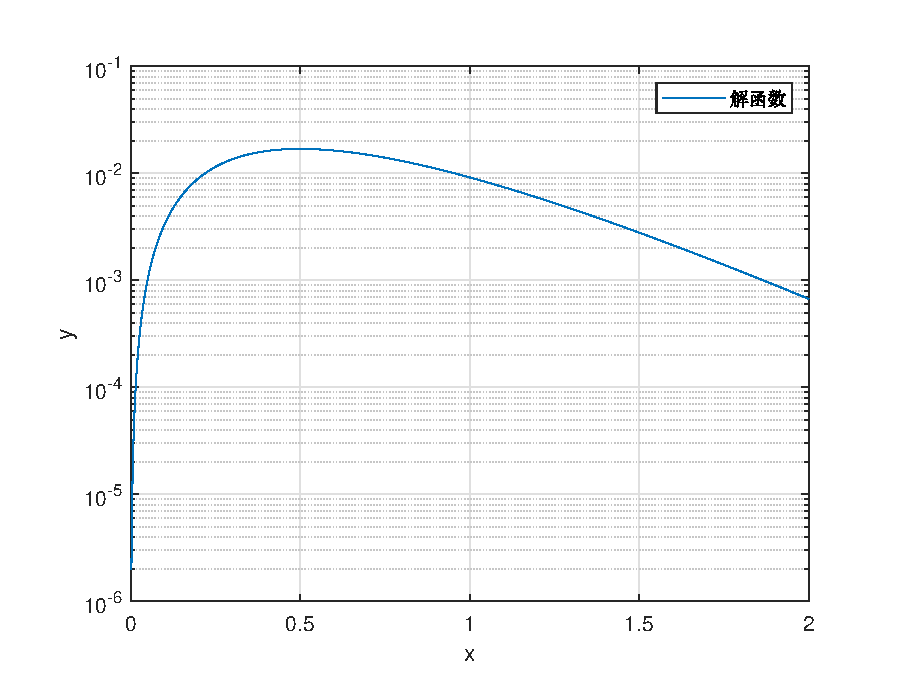
\includegraphics[scale=1]{3c.eps}
\end{center}

(d)

由题:

$\int y'dx = \int (xe^{-4x} - 4y)dx$

$\Rightarrow y = -\frac{1}{16}e^{4x}(4x + 1) - 4yx + C$

带入y(0) = 0得:

$C = \frac{1}{16}$

$\Rightarrow y = \frac{1}{16}e^{-4x} + \frac{1}{16}(4x+1)^{-1}$

在x=2这一点

err =
0.006252051077894

\textsc{Matlab}(d)程序显示如下:
\begin{lstlisting}[frame=single]
f(x) = -1/16 * exp(-4*x) + 1/16 * 1/(4*x + 1);
yk = double(yk);
err = double(abs (yk-f(2)));
format long
err
for k = 1:1001
    er(k,1) = labels(k,1);
    er(k,2) = log(abs(labels(k,2) - f((k-1)*h)))/log(h);
end
erro(er);
function erro(labels)
loglog(labels(:,1),labels(:,2));
% 记录横轴纵轴的数据画图
xlabel('x');
ylabel('精度h的log');
grid on;
legend
end
\end{lstlisting}
\begin{center}
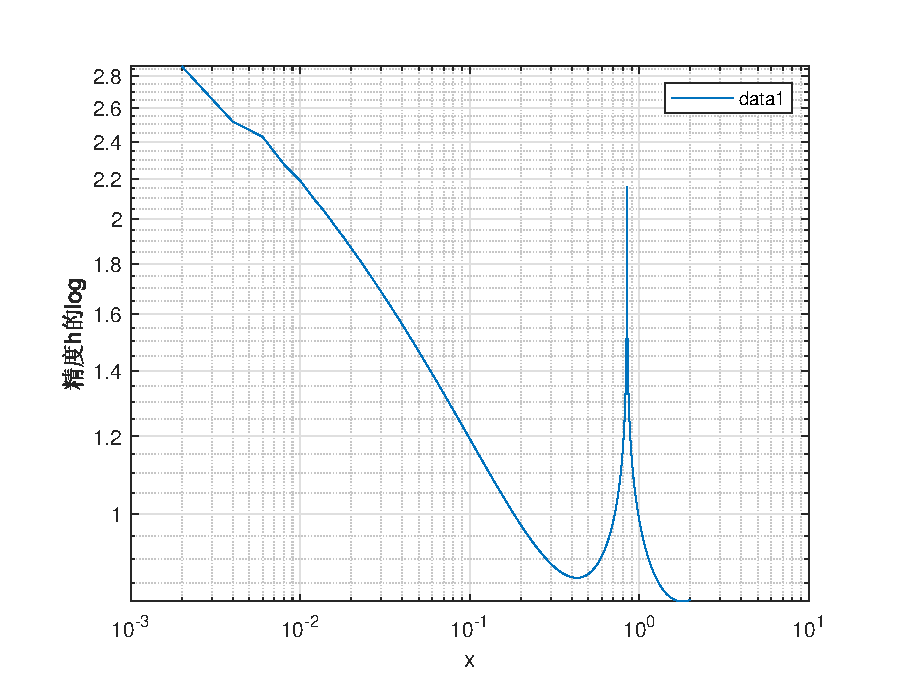
\includegraphics[scale=1]{3d.eps}
\end{center}

由于每一步需要用自身的y点进行迭代,但自身又是估计得出,因此精度和阶数达不到预期。


\end{enumerate}
\end{document}
